\documentclass[12pt]{article}

\usepackage{sbc-template}
\usepackage{graphicx,url}
\usepackage[utf8]{inputenc}
\usepackage[brazil]{babel}
\usepackage{float}
% \usepackage[latin1]{inputenc}  

     
\sloppy

\title{Comparação Entre Algoritmos de Escalonamento}

\author{Breno C. R. Nakamura\inst{1}, Estevan T. Santos\inst{1}, Gabriel L. Bonavina\inst{1}, \\
Jonas L. Durão\inst{1}, Natália V. A. do Val\inst{1}, Vinicius A. L. Andrade\inst{1}}


\address{Instituto de Ciência e Tecnologia -- Universidade Federal de São Paulo
  (UNIFESP)\\
  Av. Cesare Monsueto Giulio Lattes, 1201 -- 12247-014 -- São José dos Campos, SP
}

\begin{document} 

\maketitle

\begin{abstract}
  This meta-paper describes the style to be used in articles and short papers
  for SBC conferences. For papers in English, you should add just an abstract
  while for the papers in Portuguese, we also ask for an abstract in
  Portuguese (``resumo''). In both cases, abstracts should not have more than
  10 lines and must be in the first page of the paper.
\end{abstract}
     
\begin{resumo} 
  Este meta-artigo descreve o estilo a ser usado na confecção de artigos e
  resumos de artigos para publicação nos anais das conferências organizadas
  pela SBC. É solicitada a escrita de resumo e abstract apenas para os artigos
  escritos em português. Artigos em inglês deverão apresentar apenas abstract.
  Nos dois casos, o autor deve tomar cuidado para que o resumo (e o abstract)
  não ultrapassem 10 linhas cada, sendo que ambos devem estar na primeira
  página do artigo.
\end{resumo}

\section{Introdução}

\section{Instalação}

\section{Mudança nos Banners}

\section{Mudança \texttt{exec.c}}

\section{Descrição do Exercício Proposto}

\section{Descrição dos Algortimos de Escalonamento}

\subsection{Algoritmo Padrão do MINIX}

\subsection{Round-Robin}
O algoritmo de escalonamento por chaveamento circular (ou \textit{Round-Robin}), é um dos algoritmos 
mais simples e antigos devido à sua fácil implementação. Seu funcionamento gira em torno da definição
de uma fatia de tempo de CPU (\textit{quantum}), em que o processo que está na CPU terá um tempo limitado
de uso e, ao final deste tempo, haverá preempção e um novo processo será escolhido para ser executado \cite{tanembaum}.

\begin{figure}[H]
  \centering
  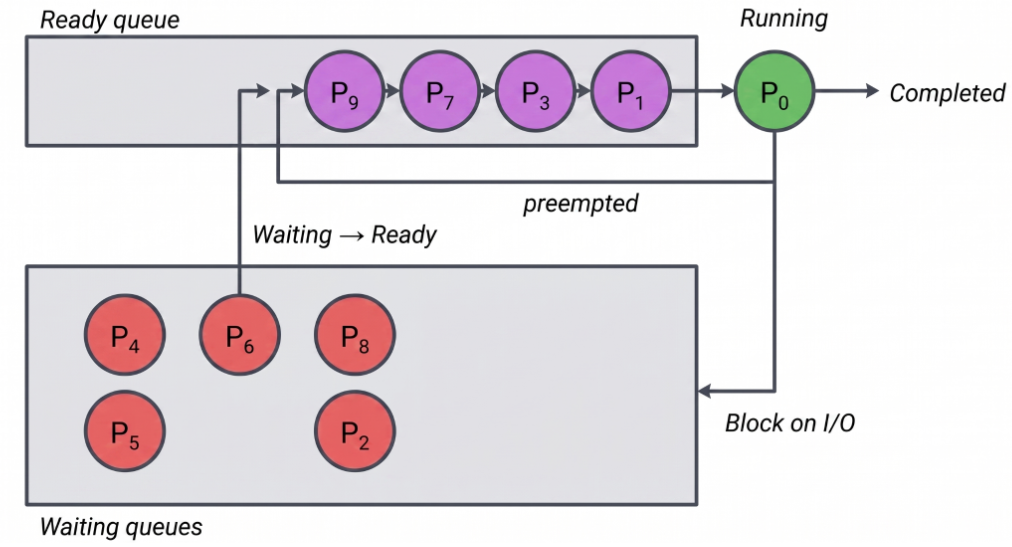
\includegraphics[width=0.5\linewidth]{round-robin.png}
  \caption{Diagrama de funcionamento do \textit{Round-Robin} \cite{slides_joahannnes}}
  \label{fig:rr}
\end{figure}

Para implementá-lo, é necessária a utilização de uma fila circular de processos prontos. Para nossa implementação,
substituimos as múltiplas filas do algoritmo padrão do MINIX por uma fila única de processos de usuário (\texttt{USER\_Q} 7),
além disso, disabilitamos os algoritmos de demoção, promoções periódicas de prioridade e rebalanceamento de filas.
Por fim, modificamos o \textit{quantum} para que ele seja variável, com a seguinte lógica: cada processo terá uma fatia de CPU
inversamente proporcional ao número de processos de usuário prontos. Em sua fila circular, quando o \textit{quantum} do processo em execução acabar, ele deverá ser encaminhado para o final da fila.
Do mesmo modo, quando ele for bloqueado por entrada e saída, quando seu estado for atualizado para pronto, ele deverá retornar ao final da fila, como pode ser visto na Figura \ref{fig:rr}.


\subsection{Múltiplas Filas}
\subsection{Algoritmo a ser escolhido}

\section{Resultados Obtidos e Discussão}

\bibliographystyle{sbc}
\bibliography{sbc-template}

\end{document}
